% Options for packages loaded elsewhere
\PassOptionsToPackage{unicode}{hyperref}
\PassOptionsToPackage{hyphens}{url}
%
\documentclass[
  10pt,
  ignorenonframetext,
]{beamer}
\usepackage{pgfpages}
\setbeamertemplate{caption}[numbered]
\setbeamertemplate{caption label separator}{: }
\setbeamercolor{caption name}{fg=normal text.fg}
\beamertemplatenavigationsymbolsempty
% Prevent slide breaks in the middle of a paragraph
\widowpenalties 1 10000
\raggedbottom
\setbeamertemplate{part page}{
  \centering
  \begin{beamercolorbox}[sep=16pt,center]{part title}
    \usebeamerfont{part title}\insertpart\par
  \end{beamercolorbox}
}
\setbeamertemplate{section page}{
  \centering
  \begin{beamercolorbox}[sep=12pt,center]{part title}
    \usebeamerfont{section title}\insertsection\par
  \end{beamercolorbox}
}
\setbeamertemplate{subsection page}{
  \centering
  \begin{beamercolorbox}[sep=8pt,center]{part title}
    \usebeamerfont{subsection title}\insertsubsection\par
  \end{beamercolorbox}
}
\AtBeginPart{
  \frame{\partpage}
}
\AtBeginSection{
  \ifbibliography
  \else
    \frame{\sectionpage}
  \fi
}
\AtBeginSubsection{
  \frame{\subsectionpage}
}

\usepackage{amsmath,amssymb}
\usepackage{iftex}
\ifPDFTeX
  \usepackage[T1]{fontenc}
  \usepackage[utf8]{inputenc}
  \usepackage{textcomp} % provide euro and other symbols
\else % if luatex or xetex
  \usepackage{unicode-math}
  \defaultfontfeatures{Scale=MatchLowercase}
  \defaultfontfeatures[\rmfamily]{Ligatures=TeX,Scale=1}
\fi
\usepackage{lmodern}
\ifPDFTeX\else  
    % xetex/luatex font selection
\fi
% Use upquote if available, for straight quotes in verbatim environments
\IfFileExists{upquote.sty}{\usepackage{upquote}}{}
\IfFileExists{microtype.sty}{% use microtype if available
  \usepackage[]{microtype}
  \UseMicrotypeSet[protrusion]{basicmath} % disable protrusion for tt fonts
}{}
\makeatletter
\@ifundefined{KOMAClassName}{% if non-KOMA class
  \IfFileExists{parskip.sty}{%
    \usepackage{parskip}
  }{% else
    \setlength{\parindent}{0pt}
    \setlength{\parskip}{6pt plus 2pt minus 1pt}}
}{% if KOMA class
  \KOMAoptions{parskip=half}}
\makeatother
\usepackage{xcolor}
\newif\ifbibliography
\setlength{\emergencystretch}{3em} % prevent overfull lines
\setcounter{secnumdepth}{-\maxdimen} % remove section numbering

\usepackage{color}
\usepackage{fancyvrb}
\newcommand{\VerbBar}{|}
\newcommand{\VERB}{\Verb[commandchars=\\\{\}]}
\DefineVerbatimEnvironment{Highlighting}{Verbatim}{commandchars=\\\{\}}
% Add ',fontsize=\small' for more characters per line
\usepackage{framed}
\definecolor{shadecolor}{RGB}{241,243,245}
\newenvironment{Shaded}{\begin{snugshade}}{\end{snugshade}}
\newcommand{\AlertTok}[1]{\textcolor[rgb]{0.68,0.00,0.00}{#1}}
\newcommand{\AnnotationTok}[1]{\textcolor[rgb]{0.37,0.37,0.37}{#1}}
\newcommand{\AttributeTok}[1]{\textcolor[rgb]{0.40,0.45,0.13}{#1}}
\newcommand{\BaseNTok}[1]{\textcolor[rgb]{0.68,0.00,0.00}{#1}}
\newcommand{\BuiltInTok}[1]{\textcolor[rgb]{0.00,0.23,0.31}{#1}}
\newcommand{\CharTok}[1]{\textcolor[rgb]{0.13,0.47,0.30}{#1}}
\newcommand{\CommentTok}[1]{\textcolor[rgb]{0.37,0.37,0.37}{#1}}
\newcommand{\CommentVarTok}[1]{\textcolor[rgb]{0.37,0.37,0.37}{\textit{#1}}}
\newcommand{\ConstantTok}[1]{\textcolor[rgb]{0.56,0.35,0.01}{#1}}
\newcommand{\ControlFlowTok}[1]{\textcolor[rgb]{0.00,0.23,0.31}{#1}}
\newcommand{\DataTypeTok}[1]{\textcolor[rgb]{0.68,0.00,0.00}{#1}}
\newcommand{\DecValTok}[1]{\textcolor[rgb]{0.68,0.00,0.00}{#1}}
\newcommand{\DocumentationTok}[1]{\textcolor[rgb]{0.37,0.37,0.37}{\textit{#1}}}
\newcommand{\ErrorTok}[1]{\textcolor[rgb]{0.68,0.00,0.00}{#1}}
\newcommand{\ExtensionTok}[1]{\textcolor[rgb]{0.00,0.23,0.31}{#1}}
\newcommand{\FloatTok}[1]{\textcolor[rgb]{0.68,0.00,0.00}{#1}}
\newcommand{\FunctionTok}[1]{\textcolor[rgb]{0.28,0.35,0.67}{#1}}
\newcommand{\ImportTok}[1]{\textcolor[rgb]{0.00,0.46,0.62}{#1}}
\newcommand{\InformationTok}[1]{\textcolor[rgb]{0.37,0.37,0.37}{#1}}
\newcommand{\KeywordTok}[1]{\textcolor[rgb]{0.00,0.23,0.31}{#1}}
\newcommand{\NormalTok}[1]{\textcolor[rgb]{0.00,0.23,0.31}{#1}}
\newcommand{\OperatorTok}[1]{\textcolor[rgb]{0.37,0.37,0.37}{#1}}
\newcommand{\OtherTok}[1]{\textcolor[rgb]{0.00,0.23,0.31}{#1}}
\newcommand{\PreprocessorTok}[1]{\textcolor[rgb]{0.68,0.00,0.00}{#1}}
\newcommand{\RegionMarkerTok}[1]{\textcolor[rgb]{0.00,0.23,0.31}{#1}}
\newcommand{\SpecialCharTok}[1]{\textcolor[rgb]{0.37,0.37,0.37}{#1}}
\newcommand{\SpecialStringTok}[1]{\textcolor[rgb]{0.13,0.47,0.30}{#1}}
\newcommand{\StringTok}[1]{\textcolor[rgb]{0.13,0.47,0.30}{#1}}
\newcommand{\VariableTok}[1]{\textcolor[rgb]{0.07,0.07,0.07}{#1}}
\newcommand{\VerbatimStringTok}[1]{\textcolor[rgb]{0.13,0.47,0.30}{#1}}
\newcommand{\WarningTok}[1]{\textcolor[rgb]{0.37,0.37,0.37}{\textit{#1}}}

\providecommand{\tightlist}{%
  \setlength{\itemsep}{0pt}\setlength{\parskip}{0pt}}\usepackage{longtable,booktabs,array}
\usepackage{calc} % for calculating minipage widths
\usepackage{caption}
% Make caption package work with longtable
\makeatletter
\def\fnum@table{\tablename~\thetable}
\makeatother
\usepackage{graphicx}
\makeatletter
\def\maxwidth{\ifdim\Gin@nat@width>\linewidth\linewidth\else\Gin@nat@width\fi}
\def\maxheight{\ifdim\Gin@nat@height>\textheight\textheight\else\Gin@nat@height\fi}
\makeatother
% Scale images if necessary, so that they will not overflow the page
% margins by default, and it is still possible to overwrite the defaults
% using explicit options in \includegraphics[width, height, ...]{}
\setkeys{Gin}{width=\maxwidth,height=\maxheight,keepaspectratio}
% Set default figure placement to htbp
\makeatletter
\def\fps@figure{htbp}
\makeatother
\newlength{\cslhangindent}
\setlength{\cslhangindent}{1.5em}
\newlength{\csllabelwidth}
\setlength{\csllabelwidth}{3em}
\newlength{\cslentryspacingunit} % times entry-spacing
\setlength{\cslentryspacingunit}{\parskip}
\newenvironment{CSLReferences}[2] % #1 hanging-ident, #2 entry spacing
 {% don't indent paragraphs
  \setlength{\parindent}{0pt}
  % turn on hanging indent if param 1 is 1
  \ifodd #1
  \let\oldpar\par
  \def\par{\hangindent=\cslhangindent\oldpar}
  \fi
  % set entry spacing
  \setlength{\parskip}{#2\cslentryspacingunit}
 }%
 {}
\usepackage{calc}
\newcommand{\CSLBlock}[1]{#1\hfill\break}
\newcommand{\CSLLeftMargin}[1]{\parbox[t]{\csllabelwidth}{#1}}
\newcommand{\CSLRightInline}[1]{\parbox[t]{\linewidth - \csllabelwidth}{#1}\break}
\newcommand{\CSLIndent}[1]{\hspace{\cslhangindent}#1}

\makeatletter
\makeatother
\makeatletter
\makeatother
\makeatletter
\@ifpackageloaded{caption}{}{\usepackage{caption}}
\AtBeginDocument{%
\ifdefined\contentsname
  \renewcommand*\contentsname{Table of contents}
\else
  \newcommand\contentsname{Table of contents}
\fi
\ifdefined\listfigurename
  \renewcommand*\listfigurename{List of Figures}
\else
  \newcommand\listfigurename{List of Figures}
\fi
\ifdefined\listtablename
  \renewcommand*\listtablename{List of Tables}
\else
  \newcommand\listtablename{List of Tables}
\fi
\ifdefined\figurename
  \renewcommand*\figurename{Figure}
\else
  \newcommand\figurename{Figure}
\fi
\ifdefined\tablename
  \renewcommand*\tablename{Table}
\else
  \newcommand\tablename{Table}
\fi
}
\@ifpackageloaded{float}{}{\usepackage{float}}
\floatstyle{ruled}
\@ifundefined{c@chapter}{\newfloat{codelisting}{h}{lop}}{\newfloat{codelisting}{h}{lop}[chapter]}
\floatname{codelisting}{Listing}
\newcommand*\listoflistings{\listof{codelisting}{List of Listings}}
\makeatother
\makeatletter
\@ifpackageloaded{caption}{}{\usepackage{caption}}
\@ifpackageloaded{subcaption}{}{\usepackage{subcaption}}
\makeatother
\makeatletter
\@ifpackageloaded{tcolorbox}{}{\usepackage[skins,breakable]{tcolorbox}}
\makeatother
\makeatletter
\@ifundefined{shadecolor}{\definecolor{shadecolor}{rgb}{.97, .97, .97}}
\makeatother
\makeatletter
\makeatother
\makeatletter
\makeatother
\ifLuaTeX
  \usepackage{selnolig}  % disable illegal ligatures
\fi
\IfFileExists{bookmark.sty}{\usepackage{bookmark}}{\usepackage{hyperref}}
\IfFileExists{xurl.sty}{\usepackage{xurl}}{} % add URL line breaks if available
\urlstyle{same} % disable monospaced font for URLs
\hypersetup{
  pdftitle={Introduction to Longitudinal Modified Treatment Policies},
  pdfauthor={Kat Hoffman},
  hidelinks,
  pdfcreator={LaTeX via pandoc}}

\title{Introduction to Longitudinal Modified Treatment Policies}
\subtitle{A solution for studying complex, continuous, and/or
time-varying exposures}
\author{Kat Hoffman}
\date{2024-02-02}

\begin{document}
\frame{\titlepage}
\ifdefined\Shaded\renewenvironment{Shaded}{\begin{tcolorbox}[interior hidden, boxrule=0pt, sharp corners, frame hidden, borderline west={3pt}{0pt}{shadecolor}, enhanced, breakable]}{\end{tcolorbox}}\fi

\begin{frame}{Overview}
\protect\hypertarget{overview}{}
\newcommand{\Pdist}{\mathsf{P}}
\newcommand{\dint}{\mathsf{d}}
\newcommand{\E}{\mathsf{E}}
\newcommand{\Ec}{\mathbb{E}}
\newcommand{\V}{\mathsf{Var}}
\newcommand{\M}{\mathcal{M}}
\newcommand{\1}{\mathbbm{1}}
\newcommand{\pr}{\mathsf{pr}}

\begin{itemize}
\tightlist
\item
  Discussing a tutorial paper on Longtudinal Modified Treatment Policies
  (accepted with minor revisions to \emph{Epidemiology})
\item
  Target audience: epidemiologists and applied statisticians
\item
  Based on methodology proposed in \emph{Díaz et al.~(2021)}
  
\includegraphics{img/jasa_ss.png}
\end{itemize}
\end{frame}

\begin{frame}{Methodology motivation}
\protect\hypertarget{methodology-motivation}{}
\begin{itemize}
\item
  Many causal inference methods and tutorials focus on binary exposures
  at a single time point

  \begin{itemize}
  \item
    Continuous/multi-level categorical exposures common in applied
    research, but methods, software, teaching materials are more limited
  \item
    Many studies have time-varying exposures, but methods are even less
    common
  \end{itemize}
\item
  Positivity assumption is essential to causal inference

  \begin{itemize}
  \item
    Violations are common in cases of categorical and continuous
    exposures
  \item
    Exacerbated when there are multiple time points
  \end{itemize}
\end{itemize}
\end{frame}

\begin{frame}{One solution: Longitudinal Modified Treatment Policies
(LMTPs)}
\protect\hypertarget{one-solution-longitudinal-modified-treatment-policies-lmtps}{}
\begin{itemize}
\item
  Diaz et al.~(2021) proposed longitudinal interventions which depend on
  an individual's \emph{natural value of treatment}

  \begin{itemize}
  \item
    Natural value of treatment: the value treatment would take at time
    \(t\) if an intervention was discontinued right before time \(t\)
  \item
    Provided identification result and doubly/sequentially robust
    estimation algoritms
  \end{itemize}
\item
  Methodology generalizes static, dynamic, and some stochastic
  interventions, so can accommodate:

  \begin{itemize}
  \tightlist
  \item
    binary, categorical, continuous, and multiple exposures
  \item
    binary, continuous, time-to-event outcomes, competing risks,
    informative right-censoring, clustering
  \item
    point-in-time and time-varying settings
  \end{itemize}
\item
  LMTPs help address violations of the positivity assumption, because we
  define an alternative interventions for which positivity holds by
  design
\end{itemize}
\end{frame}

\begin{frame}{Motivation: Tutorial}
\protect\hypertarget{motivation-tutorial}{}
\begin{enumerate}
\item
  Review static and dynamic interventions, and introduce (longitudinal)
  modified treatment policies
\item
  High-level theory:

  \begin{itemize}
  \tightlist
  \item
    Identification in point-in-time and time-varying settings
  \item
    Estimation procedures
  \end{itemize}
\item
  Application:

  \begin{itemize}
  \tightlist
  \item
    Provide examples of research questions that could be (or already
    have!) been addressed using LMTPs
  \item
    Illustrate application of an LMTP to estimate the effect of
    intubation timing on mortality in COVID-19 patients, using a
    real-world longitudinal observational data set
  \end{itemize}
\end{enumerate}
\end{frame}

\hypertarget{notation-and-setup}{%
\section{Notation and setup}\label{notation-and-setup}}

\begin{frame}{Notation}
\protect\hypertarget{notation}{}
\begin{itemize}
\item
  \(Z_1, ..., Z_n \overset{\text{iid}}{\sim} \mathsf{P}\)

  \begin{itemize}
  \item
    \(\mathsf{P}\) represents a longitudinal process and may contain any
    number of time points, but for simplicity we will describe a
    distribution with only two time points, \(t \in \{0,1\}\)
  \item
    For each unit in the study, we observe a set of random variables
    \(Z = (L_0, A_0, L_1, A_1, Y)\)
  \end{itemize}
\end{itemize}

\begin{longtable}[]{@{}
  >{\raggedright\arraybackslash}p{(\columnwidth - 4\tabcolsep) * \real{0.1538}}
  >{\raggedright\arraybackslash}p{(\columnwidth - 4\tabcolsep) * \real{0.3462}}
  >{\raggedleft\arraybackslash}p{(\columnwidth - 4\tabcolsep) * \real{0.5000}}@{}}
\toprule\noalign{}
\begin{minipage}[b]{\linewidth}\raggedright
Notation
\end{minipage} & \begin{minipage}[b]{\linewidth}\raggedright
Description
\end{minipage} & \begin{minipage}[b]{\linewidth}\raggedleft
Structural Causal Equation
\end{minipage} \\
\midrule\noalign{}
\endhead
\(L_0\) & Baseline covariates & \(L_0 \leftarrow f(U_{L_0})\) \\
\(A_0\) & Treatment at first time point &
\(f(L_0) \leftarrow U_{L_0}\) \\
\(L_1\) & Time-varying covariates & \(f(L_0) \leftarrow U_{L_0}\) \\
\(A_1\) & Treatment at second time point &
\(f(L_0) \leftarrow U_{L_0}\) \\
\(Y\) & Outcome at defined study period end &
\(f(L_0) \leftarrow U_{L_0}\) \\
\bottomrule\noalign{}
\end{longtable}
\end{frame}

\begin{frame}{Directed Acyclic Graph (DAG)}
\protect\hypertarget{directed-acyclic-graph-dag}{}
Simple DAG omitting unmeasured confounders:

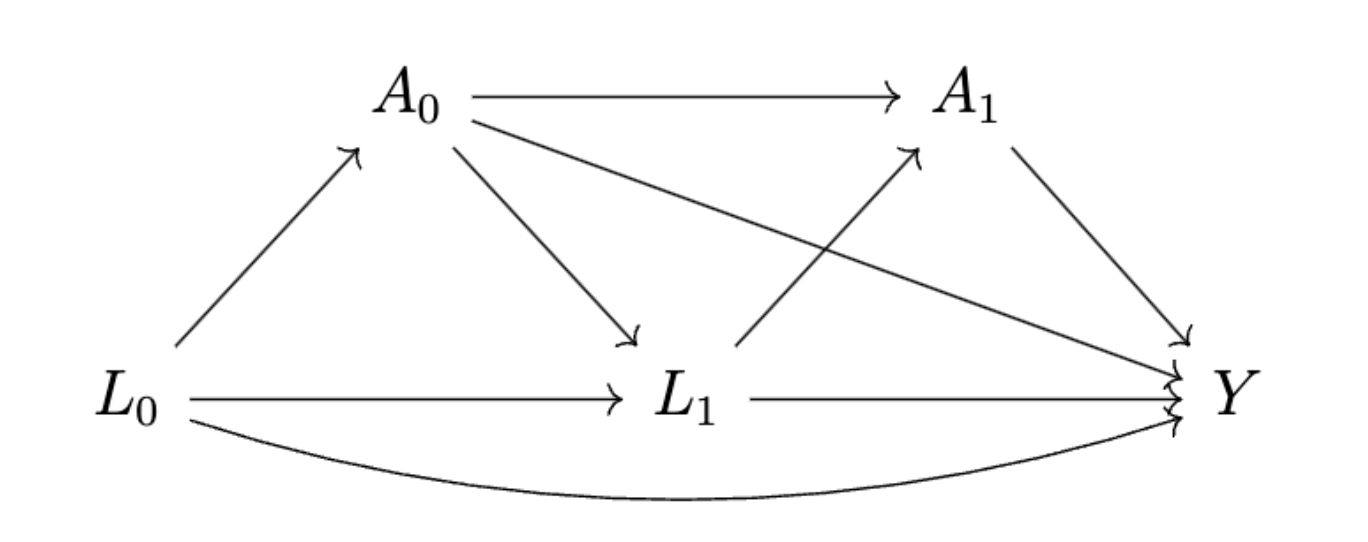
\includegraphics{img/dag.png}

Could have many more time points, high dimensional variables, competing
events, censoring nodes etc.
\end{frame}

\begin{frame}{Intervention notation}
\protect\hypertarget{intervention-notation}{}
\begin{itemize}
\item
  \(H_t\): history of data measured up to right before \(A_t\)

  \begin{itemize}
  \tightlist
  \item
    \(H_0=L_0\)
  \item
    \(H_1 = (L_0, A_0, L_1)\)
  \end{itemize}
\item
  Conceptualize treatment policies in terms of hypothetical
  interventions on nodes of the DAG
\item
  Interventions: consider a user-given function
  \(\mathsf{d}_0(a_0, h_0, \epsilon_0)\) which maps a treatment value
  \(a_0\), a history \(h_0\), and a possible randomizer \(\epsilon_0\)
  into a potential treatment value.
\end{itemize}

We refer to these longitudinal interventions, and the subsequent methods
to identify and estimate effects under such interventions, as LMTPs.
\end{frame}

\hypertarget{review-of-static-and-dynamic-interventions}{%
\section{Review of static and dynamic
interventions}\label{review-of-static-and-dynamic-interventions}}

\begin{frame}{Static interventions}
\protect\hypertarget{static-interventions}{}
\begin{itemize}
\item
  All units receive the same treatment

  \begin{itemize}
  \item
    For two time points, conceptualize a hypothetical world in which all
    units are treated at both time points \((\mathsf{d}_t = 1\) for
    \(t \in \{0, 1\})\)
  \item
    Contrast to a hypothetical world in which no units are treated at
    either time point (\(\mathsf{d}_t = 0\) \(t \in \{0, 1\})\)
  \item
    Gives rise to the well-known Average Treatment Effect (ATE)
  \end{itemize}
\end{itemize}
\end{frame}

\begin{frame}{Static intervention examples}
\protect\hypertarget{static-intervention-examples}{}
\begin{itemize}
\tightlist
\item
  Hypothetical intervening on a population to:

  \begin{itemize}
  \tightlist
  \item
    enforce 30 minutes of moderate exercise for all individuals, every
    day
  \item
    give all individuals an exact level of antibodies for a certain
    disease
  \item
    setting a certain level of air quality each day, for all
    geographical areas of interest
  \end{itemize}
\end{itemize}
\end{frame}

\begin{frame}{Dynamic interventions}
\protect\hypertarget{dynamic-interventions}{}
\begin{itemize}
\tightlist
\item
  Intervention depends only on a study unit's past covariates

  \begin{itemize}
  \tightlist
  \item
    Can include past treatment
  \end{itemize}
\item
  Often used in observational studies when study units need to meet an
  indication of interest for a treatment or policy to reasonably begin,
  e.g.

  \begin{itemize}
  \tightlist
  \item
    severity of illness indicator
  \item
    socioeconomic threshold to begin a policy
  \end{itemize}
\end{itemize}
\end{frame}

\begin{frame}{Dynamic interventions}
\protect\hypertarget{dynamic-interventions-1}{}
\begin{itemize}
\tightlist
\item
  One of the first uses of dynamic interventions was in the context of
  HIV, where investigators were interested in the effect of initiating
  antiretroviral therapy for a person with HIV if their CD4 count falls
  below a threshold, e.g.~200 cells/\(\mu\)l (Hernán et al. 2006)
\end{itemize}

\begin{align}
\mathsf{d}_t(h_t)=\begin{cases}
      1 &\text{ if } l_t^*<200 \text{ for all } s \ge t\\
      0&\text{ otherwise,}
\end{cases}
\end{align}

where \(L_t^*\) is a variable in \(H_t\) that denotes CD4 T-cell count
\end{frame}

\begin{frame}{Dynamic intervention examples}
\protect\hypertarget{dynamic-intervention-examples}{}
\begin{itemize}
\item
  Studying the effect of initiating a corticosteroids regimen for
  COVID-19 patients (Hoffman et al. 2022)
\item
  Estimated mortality under a hypothetical policy where corticosteroids
  are administered for six days if and when a COVID-19 patient first
  meets a severity of illness criteria (i.e.~low levels of blood oxygen)
\end{itemize}

\begin{align}
\mathsf{d}_t(h_t)=\begin{cases}
      1 &\text{ if } l_s^*=1 \text{ for any } s\in\{t-5,\ldots, t\}\\
      0&\text{ otherwise,}
\end{cases}
\end{align}

where \(L_t^*\) is a variable in \(H_s\) that denotes the first instance
of low levels of blood oxygen.
\end{frame}

\begin{frame}{Dynamic intervention examples}
\protect\hypertarget{dynamic-intervention-examples-1}{}
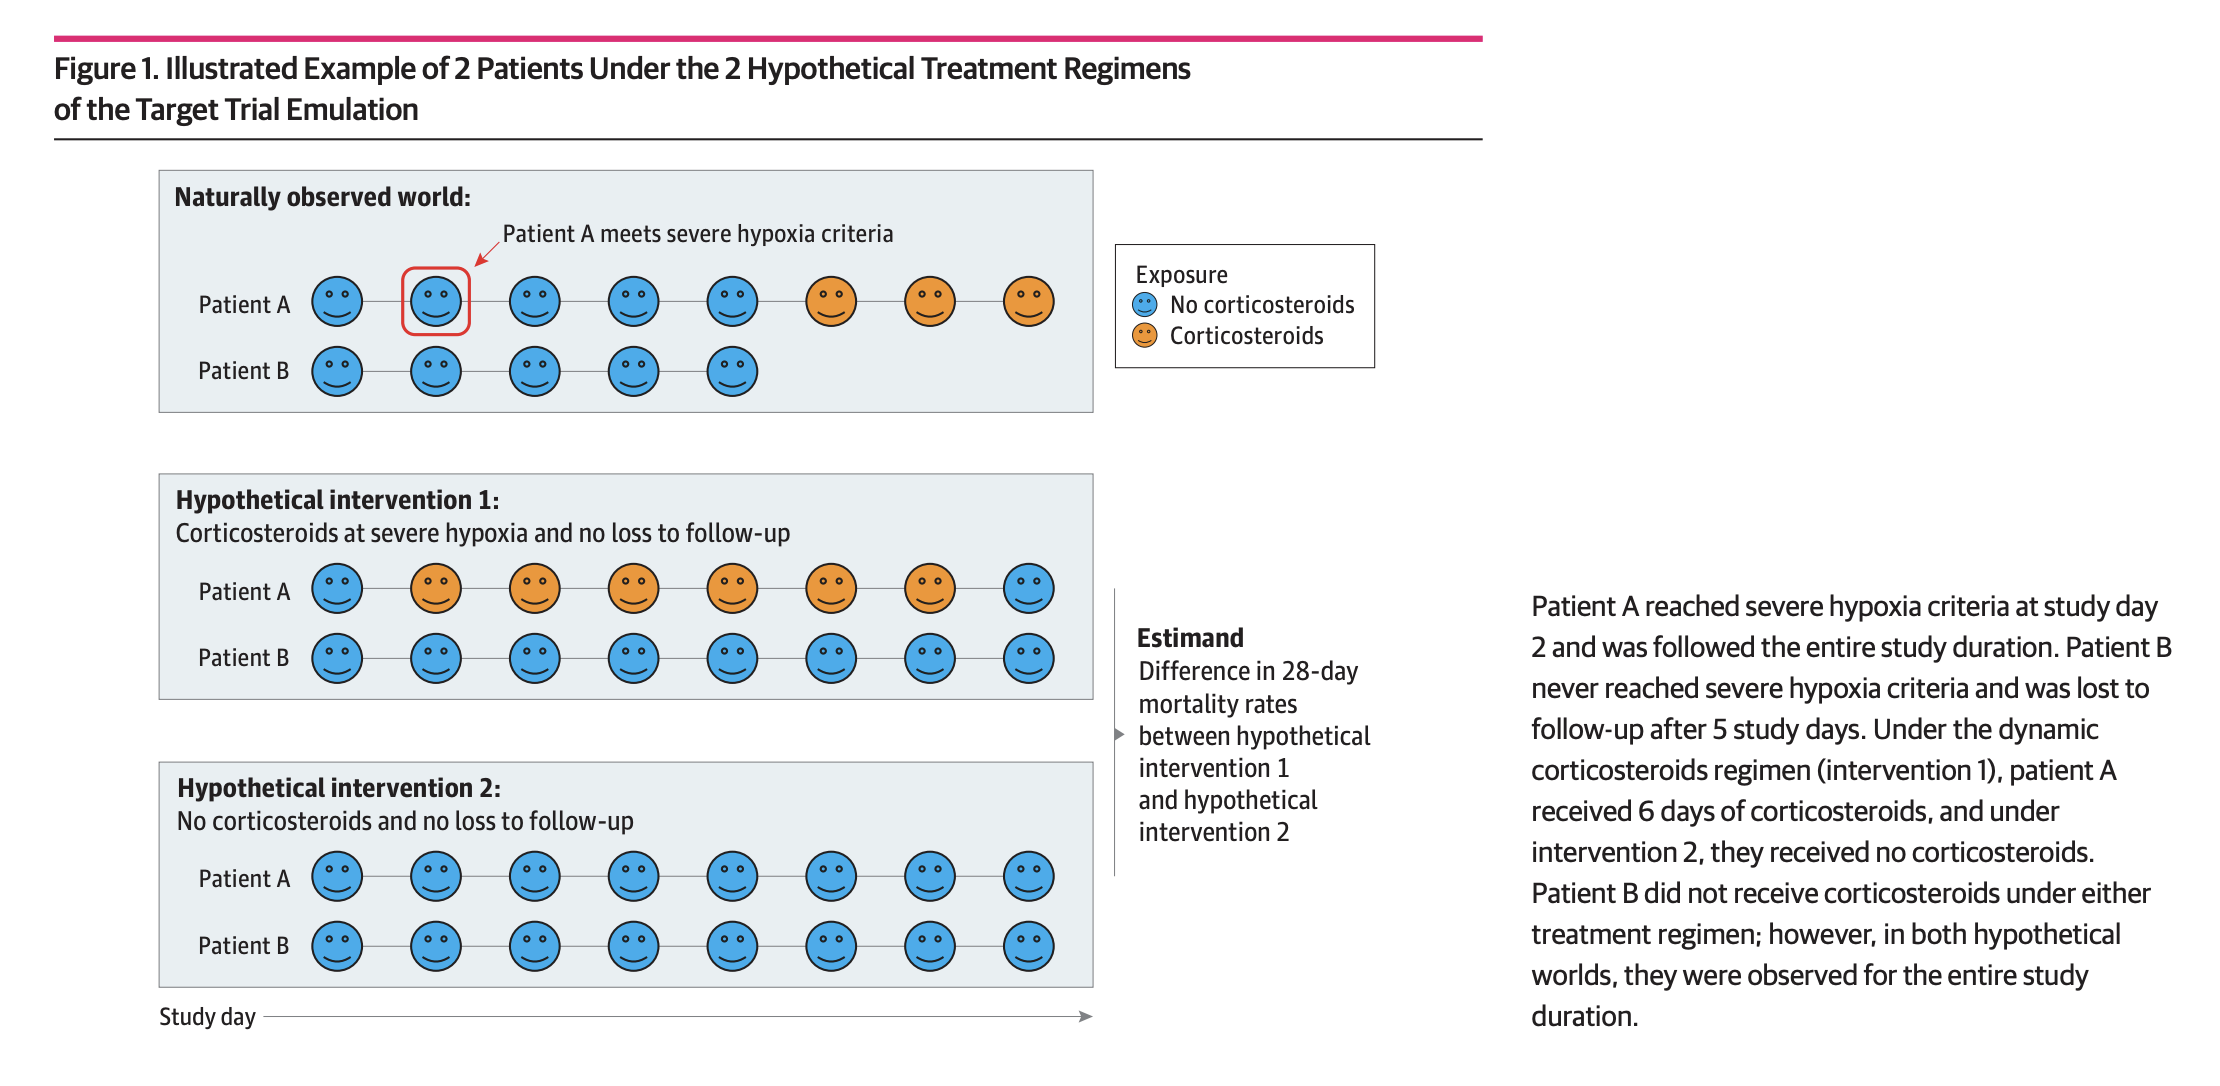
\includegraphics{img/jama_dynamic.png}
\end{frame}

\begin{frame}{Dynamic intervention examples}
\protect\hypertarget{dynamic-intervention-examples-2}{}
\begin{itemize}
\tightlist
\item
  Pollution example: instead of studying a hypothetical intervention in
  which all counties in the US have an air quality of a certain measure,
  we design a dynamic intervention in which rural counties have an air
  quality of 20 and urban counties have an air quality of 40
\end{itemize}

PICTURES
\end{frame}

\begin{frame}{Modified Treatment Policy}
\protect\hypertarget{modified-treatment-policy}{}
\begin{itemize}
\item
  Intervention function \(\d_t(a_t, h_t, \epsilon_t)\) non-trivially
  depends on the natural value of treatment \(a_t\), and perhaps on
  \(h_t\) and/or \(\epsilon_t\)
\item
  Prior examples of interventions which depend on the natural value of
  treatment

  \begin{itemize}
  \tightlist
  \item
    Threshold intervention (CITE)
  \item
    smoking cessation
  \item
    we will focus on shift interventions
  \end{itemize}
\end{itemize}
\end{frame}

\hypertarget{identification}{%
\section{Identification}\label{identification}}

\begin{frame}{Identification assumptions}
\protect\hypertarget{identification-assumptions}{}
\begin{block}{Positivity}
\protect\hypertarget{positivity}{}
\begin{itemize}
\tightlist
\item
  If it is possible to find an observation with history \(h_t\) with an
  exposure of \(a_t\), then it is also possible to find an observation
  with history \(h_t\) with an exposure \(\d(a_t, h_t, \epsilon_t)\)
\end{itemize}
\end{block}

\begin{block}{Strong sequential randomization}
\protect\hypertarget{strong-sequential-randomization}{}
\begin{itemize}
\tightlist
\item
  All common causes of the intervention variable \(A_t\) and
  \((U_{L,t+1}, U_{A,t+1})\) are measured and recorded in \(H_t\).

  \begin{itemize}
  \tightlist
  \item
    Generally satisfied if \(H_t\) contains all common causes of \(A_t\)
    and \((L_{t+1}, A_{t+1}, \ldots, L_\tau, A_\tau,\allowbreak Y)\),
    where \(\tau\) is the last time point in the study
  \end{itemize}
\end{itemize}
\end{block}

\begin{block}{Weak sequential randomizationDíaz et al. (2021)}
\protect\hypertarget{weak-sequential-randomizationrichardson2013single-diaz_nonparametric_2021}{}
\begin{itemize}
\tightlist
\item
  All common causes of the intervention variable \(A_t\) and
  \((U_{L,t+1})\) are measured and recorded in \(H_t\) (Taubman et al.
  2009)
\end{itemize}
\end{block}
\end{frame}

\begin{frame}{Identification formula}
\protect\hypertarget{identification-formula}{}
\begin{enumerate}

\item Start with the conditional expectation of the outcome $Y$ given $A_1=a_1$ and $H_1=h_1$. Let this function be denoted $Q_1(a_1, h_1)$.
\item Evaluate the above conditional 
  expectation of $Y$ if $A_1$ were changed to $A^\mathsf{d}_1$, which results in 
  a pseudo outcome $\tilde Y_1=Q_1(A^\mathsf{d}_1, H_1)$.
\item Let the true expectation of $\tilde Y_1$ conditional on
  $A_0=a_0$ and $H_0=h_0$ be denoted $Q_0(a_0, h_0)$.
\item Evaluate the above
  expectation of $\tilde Y_1$ if $A_0$ were changed to $A^\mathsf{d}_0$, which results in
  $\tilde Y_0=Q_0(A^\mathsf{d}_0, H_0)$.
\item Under the identifying assumptions, we have
  $\mathsf{E}[Y(\bar{A}_\tau^\mathsf{d})]=\mathsf{E}[\tilde Y_0]$.
  
\end{enumerate}
\end{frame}

\hypertarget{estimation}{%
\section{Estimation}\label{estimation}}

\begin{frame}{test}
\protect\hypertarget{test}{}
Once a causal estimand is defined and identified, the researcher's task
is to estimate the statistical quantity,
e.g.~\(\mathsf{E}[\Tilde{Y}_0]\)
\end{frame}

\begin{frame}{Parametric estimation}
\protect\hypertarget{parametric-estimation}{}
\begin{itemize}
\tightlist
\item
  Simplest option: fit parametric outcome regressions for each step of
  g-formula identification result

  \begin{itemize}
  \tightlist
  \item
    ``Plug-in'' estimator called \textbf{parametric g-formula} or
    \textbf{g-computation}
  \end{itemize}
\item
  Alternatively, use estimator which relies on the exposure mechanism

  \begin{itemize}
  \tightlist
  \item
    Inverse Probability Weighting (IPW) estimator
  \item
    IPW estimation involves reweighting the observed outcome by a
    quantity which represents the likelihood the intervention was
    received, conditional on covariates
  \end{itemize}
\end{itemize}
\end{frame}

\begin{frame}{G-computation}
\protect\hypertarget{g-computation}{}
\begin{enumerate}
\item Fit a generalized linear model (GLM) for $Y$ conditional on $A_1=a_1$ and
  $H_1=h_1$. Call this $\hat{Q_1}(a_1, h_1)$.
  
  \texttt{Q1\_hat} $\gets$ \texttt{glm}$(\text{outcome} = Y, \text{predictors} = \{H_1, A_1\})$


\item Modify the data set used in step (1) so that the values in the column for $A_1$ are changed to $A^\mathsf{d}_1$. Obtain the predictions for the model $\hat{Q_1}$ using this modified data set. These are pseudo-outcomes
  $\tilde Y_1$.

\texttt{pseudo\_Y1} $\gets$ \texttt{predict}$(\text{fit} =   \texttt{Q1\_hat}, \text{new data} = \{H_1, A_1 = A_1^\mathsf{d}\} )$

\item Fit a generalized linear model (GLM) for $\tilde Y_1$ conditional on
  $A_0=a_0$ and $H_0=h_0$. Call this $\hat{Q_0}(a_0, h_0)$.

  \texttt{Q0\_hat} $\gets$ \texttt{glm}$(\text{outcome} = \texttt{pseudo\_Y1}, \text{predictors} = \{H_0, A_0\})$

\item  Modify the data set used in step (3) so that the values in the column for $A_0$ are changed to $A^\mathsf{d}_0$. Obtain the predictions for the model $\hat{Q_0}$ using this modified data set. These are pseudo-outcomes
  $\tilde Y_0$.

\texttt{pseudo\_Y0} $\gets$ \texttt{predict}$(\text{fit} =   \texttt{Q1\_hat}, \text{new data} = \{H_0, A_0 = A_0^\mathsf{d}\} )$

\item Average $\tilde Y_0$, i.e. compute $\hat\mathsf{E}[\tilde Y_0]$.

\texttt{estimate} $\gets$ \texttt{mean(pseudo\_Y0)}
\end{enumerate}
\end{frame}

\begin{frame}{Temp}
\protect\hypertarget{temp}{}
--\textgreater{}
\end{frame}

\begin{frame}{Application examples}
\protect\hypertarget{application-examples}{}
\end{frame}

\begin{frame}{Illustrative application}
\protect\hypertarget{illustrative-application}{}
\end{frame}

\begin{frame}{Software/algos}
\protect\hypertarget{softwarealgos}{}
\end{frame}

\begin{frame}{Technicalities}
\protect\hypertarget{technicalities}{}
Or \textbf{bold}, \emph{italic}, or \href{https://illinois.edu}{URL}
text.
\end{frame}

\begin{frame}{Mathematics}
\protect\hypertarget{mathematics}{}
Inline mode: \(c^2 = a^2 + b^2\)

Display mode:

\[x = \frac{-b \pm \sqrt{b^2 - 4ac}}{2a}\]
\end{frame}

\begin{frame}{Columns}
\protect\hypertarget{columns}{}
We could also split content between two columns:

\begin{columns}[T]
\begin{column}{0.45\textwidth}
Left column
\end{column}

\begin{column}{0.45\textwidth}
Right column
\end{column}
\end{columns}

\url{https://quarto.org/docs/presentations/revealjs/\#multiple-columns}
\end{frame}

\begin{frame}[fragile]{Code Highlighting}
\protect\hypertarget{code-highlighting}{}
For continuous highlighting, use \texttt{from-to} (\texttt{6-8}).

For discontinuous highlighting, use \texttt{line1,\ line2,\ ...}
(\texttt{1,\ 4}).

To highlight lines in a progressive manner, use
\texttt{range1\textbar{}range2} (\texttt{\textbar{}1,4\textbar{}6-8}).

\begin{Shaded}
\begin{Highlighting}[numbers=left,,]
\ImportTok{import}\NormalTok{ numpy }\ImportTok{as}\NormalTok{ np}
\ImportTok{import}\NormalTok{ matplotlib.pyplot }\ImportTok{as}\NormalTok{ plt}

\NormalTok{r }\OperatorTok{=}\NormalTok{ np.arange(}\DecValTok{0}\NormalTok{, }\DecValTok{2}\NormalTok{, }\FloatTok{0.01}\NormalTok{)}
\NormalTok{theta }\OperatorTok{=} \DecValTok{2} \OperatorTok{*}\NormalTok{ np.pi }\OperatorTok{*}\NormalTok{ r}
\NormalTok{fig, ax }\OperatorTok{=}\NormalTok{ plt.subplots(subplot\_kw}\OperatorTok{=}\NormalTok{\{}\StringTok{\textquotesingle{}projection\textquotesingle{}}\NormalTok{: }\StringTok{\textquotesingle{}polar\textquotesingle{}}\NormalTok{\})}
\NormalTok{ax.plot(theta, r)}
\NormalTok{ax.set\_rticks([}\FloatTok{0.5}\NormalTok{, }\DecValTok{1}\NormalTok{, }\FloatTok{1.5}\NormalTok{, }\DecValTok{2}\NormalTok{])}
\NormalTok{ax.grid(}\VariableTok{True}\NormalTok{)}
\NormalTok{plt.show()}
\end{Highlighting}
\end{Shaded}

\url{https://quarto.org/docs/presentations/revealjs/\#code-blocks}
\end{frame}

\begin{frame}[fragile]{Enable more revealjs features}
\protect\hypertarget{enable-more-revealjs-features}{}
The theme is built ontop of Quarto's \texttt{revealjs} implementation.
So, any \href{https://quarto.org/docs/presentations/revealjs/}{features}
of available are also usable within the theme. For example, if we wanted
to incorporate the
\href{https://quarto.org/docs/presentations/revealjs/presenting.html\#chalkboard}{chalkboard}
feature. We would use:

\begin{Shaded}
\begin{Highlighting}[]
\FunctionTok{format}\KeywordTok{:}
\AttributeTok{  }\FunctionTok{washington{-}revealjs}\KeywordTok{:}\AttributeTok{ }
\AttributeTok{    }\FunctionTok{chalkboard}\KeywordTok{:}\AttributeTok{ }\CharTok{true}
\end{Highlighting}
\end{Shaded}
\end{frame}

\begin{frame}[fragile]{Summary}
\protect\hypertarget{sec-summary}{}
\begin{block}{UW-themed presentation slide deck}
\protect\hypertarget{uw-themed-presentation-slide-deck}{}
The Quarto University of Washington Revealjs theme is an extension of
Reveal.js and offers all of its
\href{https://quarto.org/docs/presentations/revealjs/}{features} in the
context of being brand friendly at UW.

Install the theme without this template:

\begin{Shaded}
\begin{Highlighting}[]
\ExtensionTok{quarto}\NormalTok{ install extension kathoffman/quarto{-}uw}
\end{Highlighting}
\end{Shaded}

Install the theme with the template being present:

\begin{Shaded}
\begin{Highlighting}[]
\ExtensionTok{quarto}\NormalTok{ use template kathoffman/quarto{-}uw}
\end{Highlighting}
\end{Shaded}

You can learn more about using RevealJS with Quarto at:
\url{https://quarto.org/docs/presentations/revealjs/}

\hypertarget{refs}{}
\begin{CSLReferences}{1}{0}
\leavevmode\vadjust pre{\hypertarget{ref-diaz_nonparametric_2021}{}}%
Díaz, Iván, Nicholas Williams, Katherine L. Hoffman, and Edward J.
Schenck. 2021. {``Nonparametric {Causal} {Effects} {Based} on
{Longitudinal} {Modified} {Treatment} {Policies}.''} \emph{Journal of
the American Statistical Association}, September, 1--16.
\url{https://doi.org/10.1080/01621459.2021.1955691}.

\leavevmode\vadjust pre{\hypertarget{ref-hernan2006comparison}{}}%
Hernán, Miguel A, Emilie Lanoy, Dominique Costagliola, and James M
Robins. 2006. {``Comparison of Dynamic Treatment Regimes via Inverse
Probability Weighting.''} \emph{Basic \& Clinical Pharmacology \&
Toxicology} 98 (3): 237--42.

\leavevmode\vadjust pre{\hypertarget{ref-hoffman2022comparison}{}}%
Hoffman, Katherine L, Edward J Schenck, Michael J Satlin, William
Whalen, Di Pan, Nicholas Williams, and Iván Dı́az. 2022. {``Comparison of
a Target Trial Emulation Framework Vs Cox Regression to Estimate the
Association of Corticosteroids with COVID-19 Mortality.''} \emph{JAMA
Network Open} 5 (10): e2234425--25.

\leavevmode\vadjust pre{\hypertarget{ref-richardson2013single}{}}%
Richardson, Thomas S, and James M Robins. 2013. {``Single World
Intervention Graphs (SWIGs): A Unification of the Counterfactual and
Graphical Approaches to Causality.''} \emph{Center for the Statistics
and the Social Sciences, University of Washington Series. Working Paper}
128 (30): 65--78.

\leavevmode\vadjust pre{\hypertarget{ref-taubman2009intervening}{}}%
Taubman, Sarah L, James M Robins, Murray A Mittleman, and Miguel A
Hernán. 2009. {``Intervening on Risk Factors for Coronary Heart Disease:
An Application of the Parametric g-Formula.''} \emph{International
Journal of Epidemiology} 38 (6): 1599--1611.

\end{CSLReferences}
\end{block}
\end{frame}



\end{document}
